\begin{figure}
\centering
\begin{subfigure}{.5\textwidth}
  \centering
  
\includegraphics[width=.95\linewidth]{../study-2/results/visualisations/didactic-one.png}
  \caption{Phase 1}
  \label{fig:didactic-one}
\end{subfigure}%
\begin{subfigure}{.5\textwidth}
  \centering
  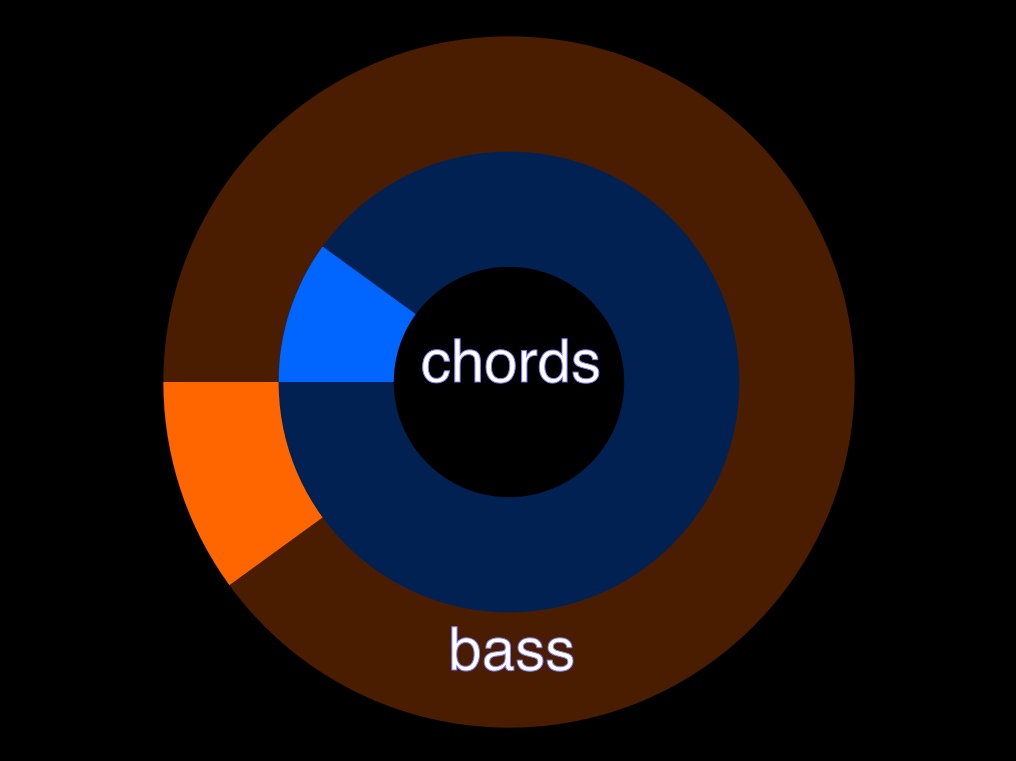
\includegraphics[width=.95\linewidth]{../study-2/results/visualisations/didactic-two.png}
  \caption{Phase 2}
  \label{fig:didactic-two}
\end{subfigure}\\
\begin{subfigure}{.5\textwidth}
  \centering
  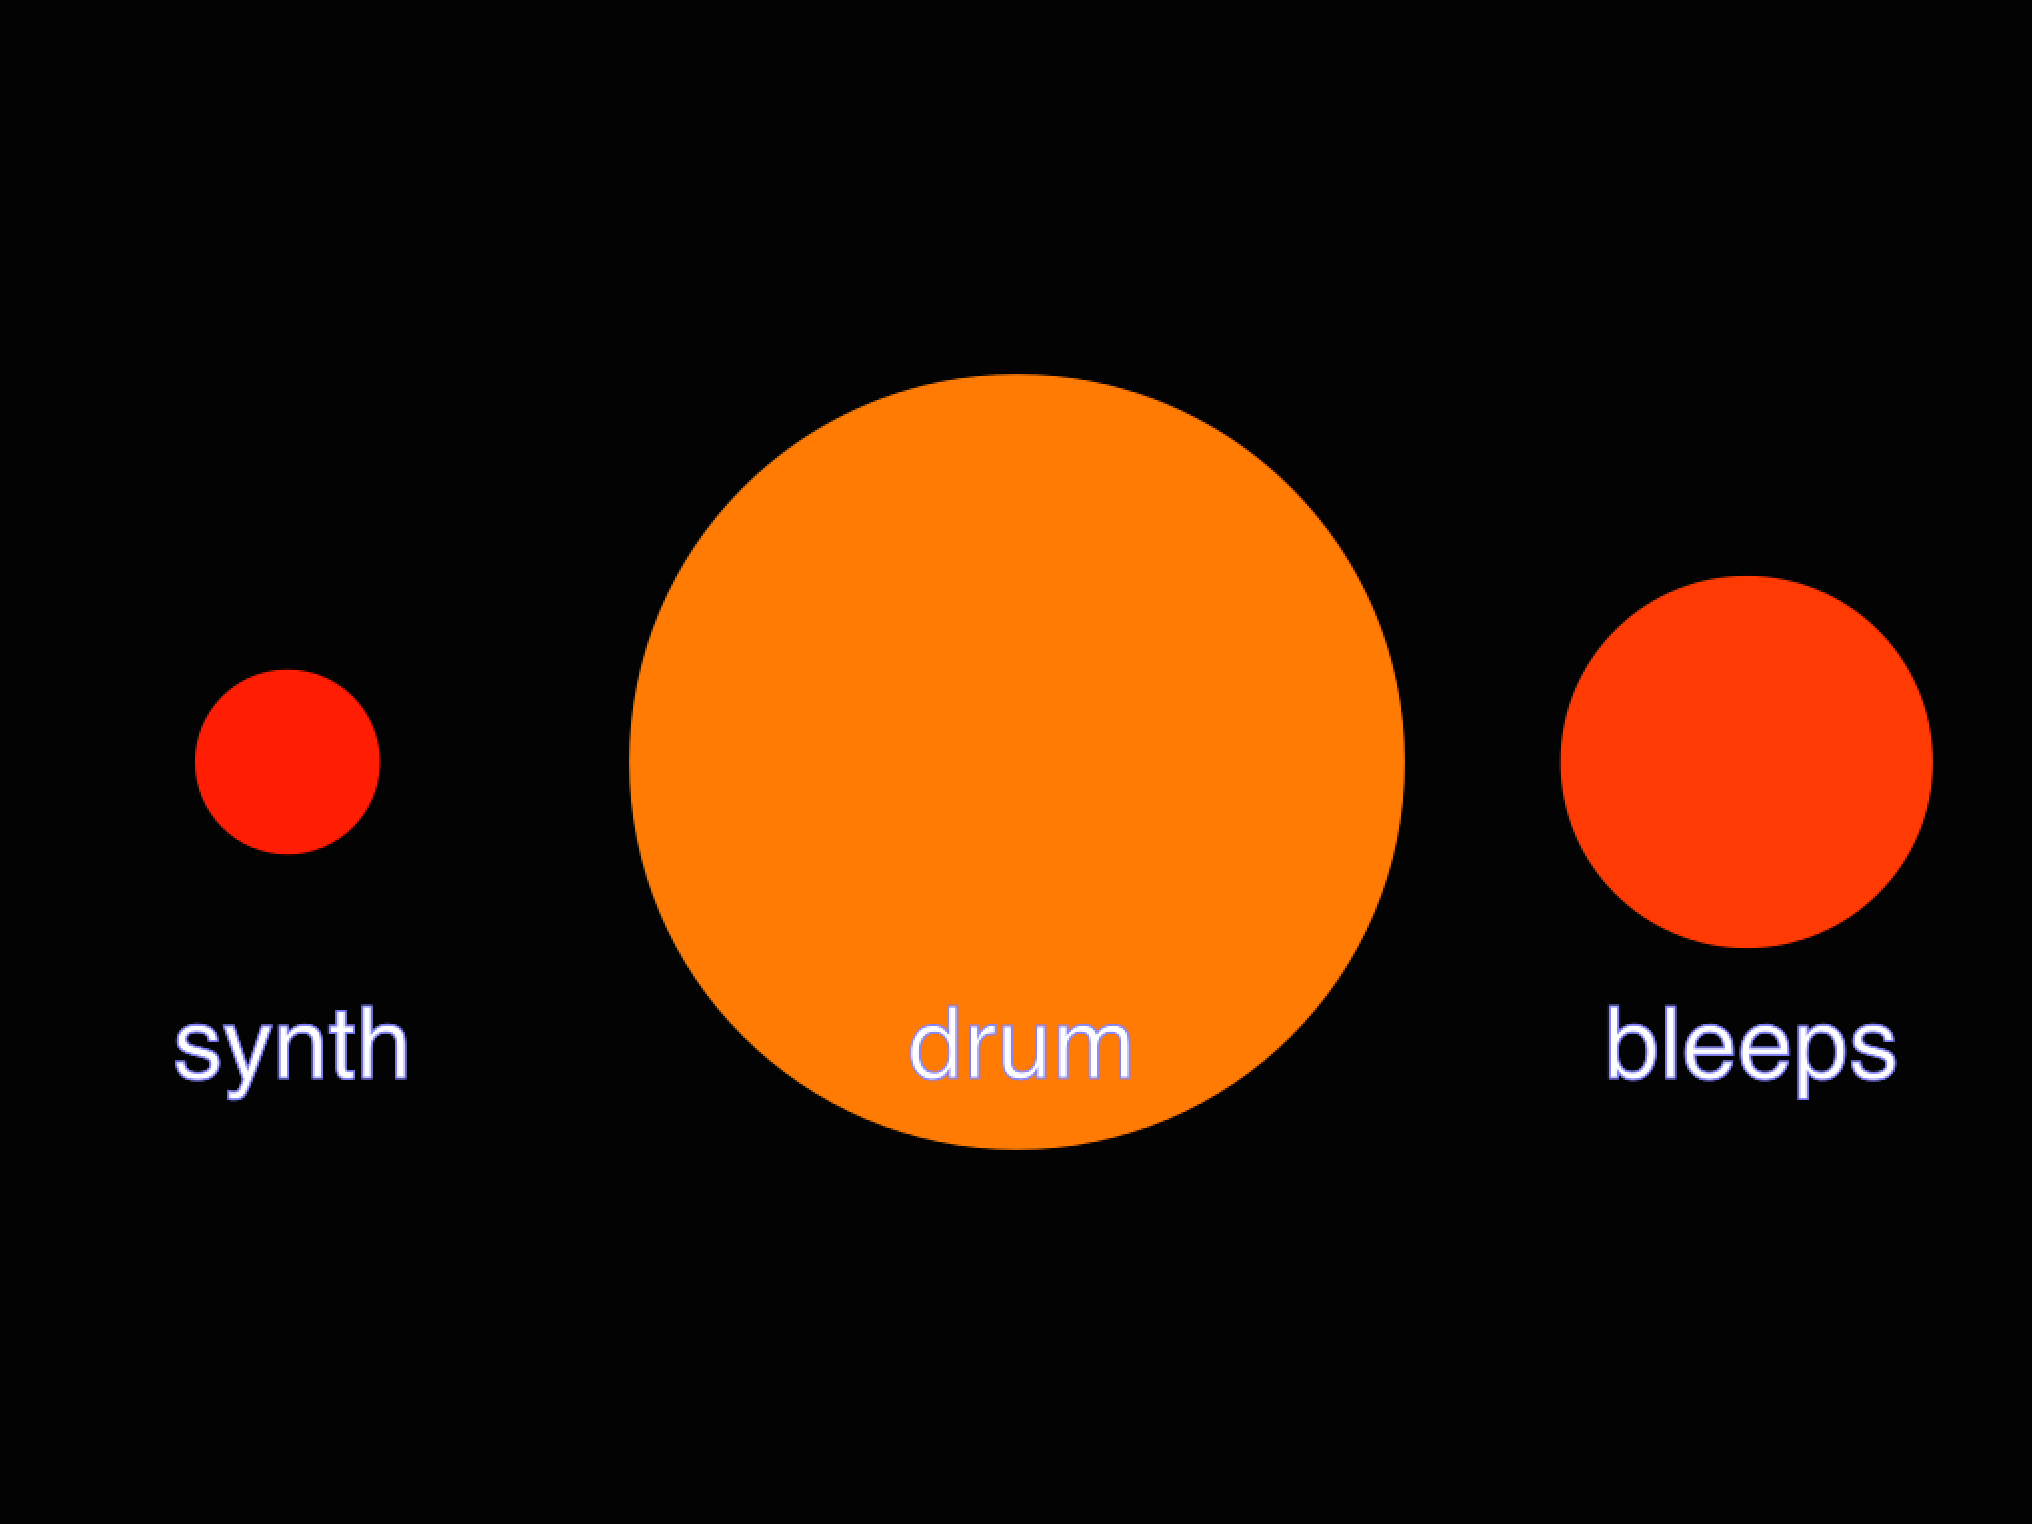
\includegraphics[width=.95\linewidth]{../study-2/results/visualisations/didactic-three.png}
  \caption{Phase 3}
  \label{fig:didactic-three}
\end{subfigure}%
\begin{subfigure}{.5\textwidth}
  \centering
  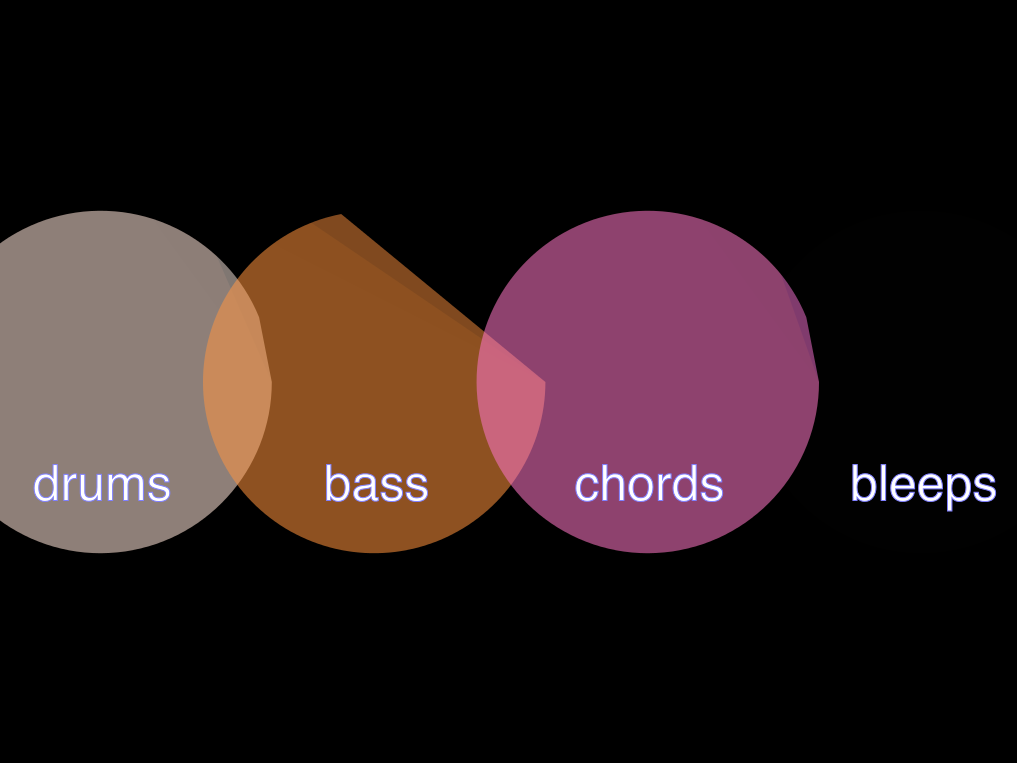
\includegraphics[width=.95\linewidth]{../study-2/results/visualisations/didactic-four.png}
  \caption{Phase 4}
  \label{fig:didactic-four}
\end{subfigure}

\caption[Didactic visualisation phases]{The four phases of the didactic visualisation.}
\label{fig:didactic-visualisations}
\end{figure}
